\documentclass[a4paper,10pt]{article}
\usepackage[utf8]{inputenc}
\usepackage{xspace}
\usepackage{graphicx,graphics} 
\usepackage{color}
\usepackage{amsmath}
\usepackage{amsfonts}
\usepackage{amssymb}
\usepackage{amsthm}
\usepackage{algorithm}
\usepackage{algorithmic}
\usepackage{longtable}
\usepackage{complexity}
\usepackage{tkz-graph}
\usepackage{float}
\usepackage{setspace}
\renewcommand{\algorithmicrequire}{\textbf{Input:}}
\renewcommand{\algorithmicensure}{\textbf{Output:}}
  
\graphicspath{{figures/}}
\newcommand\rmatching{${\cal R}$-matching\xspace}
\newcommand\mdelay{$\cal M$-delay\xspace}
\newcommand\matchedgraph{{\bf matched graph}}
\newtheorem{proposition}{Proposition}
\newtheorem{theorem}{Theorem}
\newcommand{\reporttitle}{Contention management for Deterministic Networking}     % Titre
\newcommand{\reportauthor}{Maël \textsc{Guiraud }} % Auteur
\newcommand{\reportsubject}{Master Thesis} 
\newcommand{\HRule}{\rule{\linewidth}{0.5mm}}
\setlength{\parskip}{1ex} % Espace entre les paragraphes


\newcommand{\todo}[1]{{\color{red} TODO: {#1}}}


%opening
\title{Contention Management for 5G}
\author{DB,CC,MG,OM,YS}


\begin{document}

\maketitle

\begin{abstract}
This article treats about Contention Management for 5G.
\end{abstract}

\section{Introduction}
  \itemize
    \item Context and problematic
    \item Related works
    \item Article contribution

\section{Model, Problems}

  \subsection{Definitions}
	  A network can be considered as a directed graph $G=(V,A)$ with two non intersecting subsets of vertices: 
	a subset $L$ of nodes which are called {\bf leaves} and a subset $S$ of nodes which are called {\bf sources}.  
      The indegree of nodes in $S$, and the outdegree of nodes in $L$ are equal to 0. 
      We denote by ${\cal L}$ the cardinal of $L$ and by ${\cal S}$ the cardinal of $S$. 
      Each arc  $(u,v)$ in $A$ has an integer weight $Dl(u,v)$, called {\bf delay}, representing the time taken by a data to go from $u$ to $v$
      using this arc.

      We consider $G^r=(V,A^r)$ wherein the set of vertices is the same as in $G$, and $A^r$ represents the edges of $A$ directed in the other way. 
      \newline
      \begin{center}
      \fbox{\parbox{11cm}{
      \begin{figure}[H]
      \begin{center}
      \begin{tabular}{cc}
      \includegraphics[scale=0.8]{Fig2.pdf} & \includegraphics[scale=0.8]{Fig3.pdf}\\
      $G=(V,A)$ & $G^r=(V,A^r)$\\
      \end{tabular}
      \end{center}
      \caption{$G$ and $G^r$ with ${\cal L} = {\cal S} = 1$.}
      \end{figure}

      }}\end{center}

      A {\bf route} $r$ is a sequence of arcs $a_0, \ldots , a_{n-1}$, with $a_i=(u_i,u_{i+1}) \in A$ such that $u_0 \in L$ and $u_n \in S$.
      The delay of a vertex $u_i$ in $r$, with $i \geq 1$, is defined by $$\lambda(u_i,r)= \sum\limits_{0 \leq k <i} Dl(a_k)$$ We also define $\lambda(u_0,r)=0$.
      The delay of the route $r$ is defined by $\lambda (r)= \lambda (u_n,r)$. It is the weight of all the arcs on the route.

      A {\bf routing function}  ${\cal R}$ is an application associating a route  ${\cal R}(s,l)$ to each couple $(s,l) \in S \times L$ in $G$.
      Moreover ${\cal R}$ satisfies the {\bf coherent routing} property: the intersection of two routes must be a path.

      For simplicity, we assume that we have as many source nodes as we have leaves (${\cal S} = {\cal L})$.
      A {\bf ${\cal R}$-matching} is a bijection $\rho:S\rightarrow L$ which associates to each $s_i \in \{s_0,...,s_{{\cal S}-1}\}$ 
      a $l_i \in \{l_0,...,l_{{\cal L}-1}\}$.
      A \rmatching defines a set $\{r_0, \ldots ,r_{{\cal L}-1}\}$ of ${\cal L}$ routes in ${\cal R}$ such that $\forall i\,, r_i = {\cal R}(s_i,l_i)$.

      The quintuplet $N=(G,S,L,{\cal R},\rho)$ defines a \matchedgraph. We call $N^r$ the quintuplet $(G^r,S,L,{\cal R},\rho^r)$, 
      where $\rho^r$ is the \rmatching obtained using the same routes, with inverted arcs.

    
      \subsection{Slotted time Model}
      \label{slottedtime}
      In our model, the time is discrete. The unit of time is one slot. Two values are expressed in time slots: 
      \enumerate
      \item The emission time of a message by a node, the {\bf message length}, We denote by {\bf T} this time.
      \item The time taken by a message to cross a link, the delay of an arc.


      Let $P>0$ be an integer called {\bf period}. 
      A {\bf $P$-periodic affectation} of $N$(a matched graph) consists in a set  ${\cal M}=(m_0, \ldots ,m_{{\cal L}-1})$
      of ${\cal L}$ integers that we call {\bf offset}. 
      Each period is divided in $P$ slots and the number $m_i$ represents the first slot number used by the route $r_i$ at its source.
      We define the first time slot at which a message arrive at any vertex $v$ of the route by $$t(v,r_i) = m_i+\lambda(u,r_i) \mod P.$$

      Let us call $[t(v,r_i)]_{T,P}$ the values of the time slots used by a route $r_i$ in a vertex $v$. 
      Those values are forming a continuous set of values starting at $t(v,r_i) \mod P$ and ending at $t(v,r_i) + T \mod P$.
      For a given instance, $P$ and T does not change at any moment, indeed, the size of the messages is the same for any route, and the period is also the same for any vertex.
      So, since $P$ and T are fixed, we simplify the notation by $[t(v,r_i)]$.

      A $P$-periodic affectation must have no {\bf collision} between two routes in $\rho$, that is $\forall r_i, r_j \in \rho, i \ne j$,
      we have $$[t(u,r_i)] \cap [t(u,r_j)] = \emptyset .$$

   
  
  \subsection{Problems}
	
    The application we address here by studying the problems defined above is the following. Consider a fronthaul network in which source nodes in $S$ represent BBU.
    Each of the source nodes do a computation for its associated RRH represented by a leaf node in $L$. Consider a ${\cal R}$-matching $\rho$ of $S$ in $L$. Consider a leaf $l$, its dedicated source node $s$
    and $R(l,s)$ the route from $l$ to $s$ in $R$. We consider a $P$-periodic affectation of N, and also another $P$-periodic affectation of $N^{r}$.
    The periodic process is, for each route, the following one:
    \begin{enumerate}
    \item During each period of duration $P$, $l$ sends a message to its source $s=\rho(l)$, using its routes according to the $P$-periodic affectation of N. 
    \item When a source $s=\rho(l)$ receive a message from $l$, it makes a computation. This computation time is the same for all sources.
    \item After this computation time, $s$ sends a message to $l=\rho(l)$ according to the $P$-periodic affectation of $N^{r}$.
    \end{enumerate}

    \begin{center}
    \fbox{\parbox{11cm}{
    \begin{figure}[H]
    \begin{center}
    \scalebox{0.6}{
    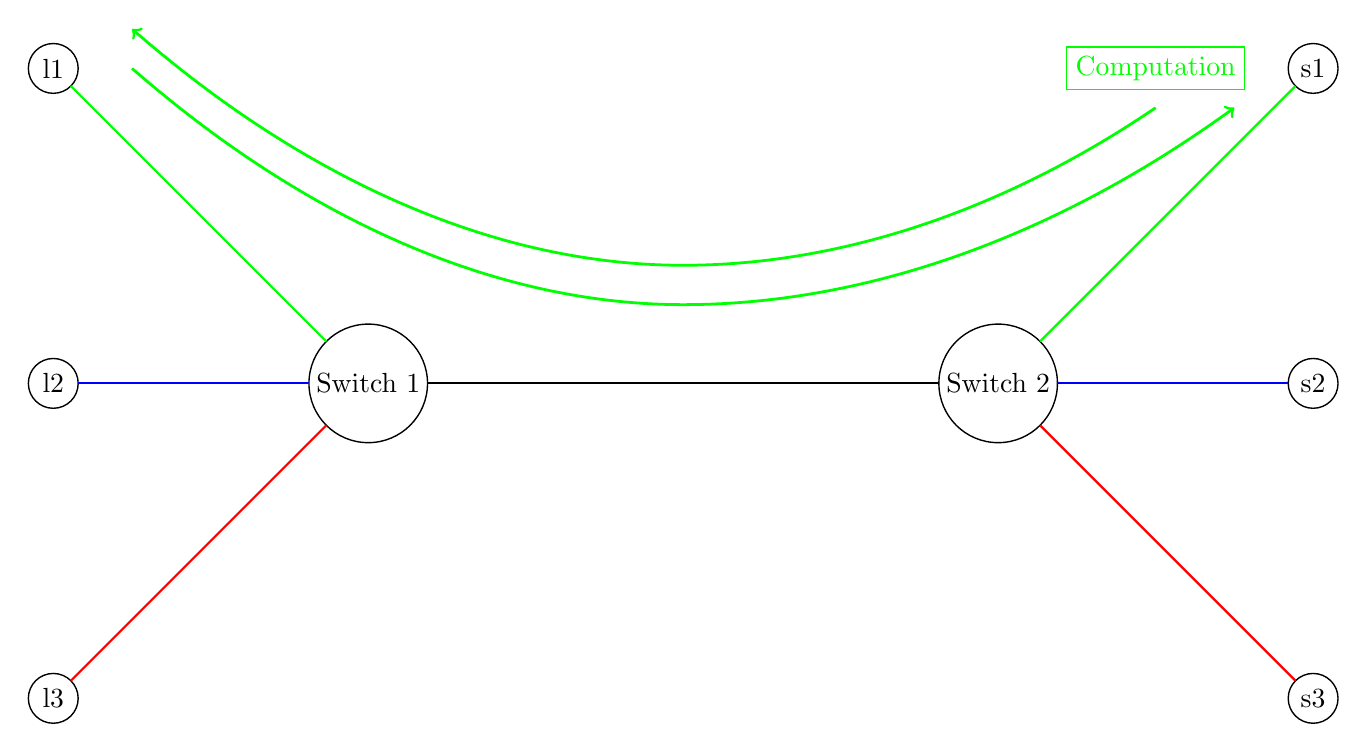
\begin{tikzpicture}
      \SetGraphUnit{5}
      \Vertex[x=0,y=0]{l3}
      \Vertex[x=0,y=4]{l2}
      \Vertex[x=0,y=8]{l1}
      
      \Vertex[x=16,y=0]{s3}
      \Vertex[x=16,y=4]{s2}
      \Vertex[x=16,y=8]{s1}
      
      \Vertex[x=4,y=4]{Switch 1}
      \Vertex[x=12,y=4]{Switch 2}  
      \tikzset{
      EdgeStyle/.append style = {green} }
      \Edge(s1)(Switch 2)
      \Edge(Switch 1)(l1)
      
      \tikzset{
      EdgeStyle/.append style = {blue} }
      \Edge(s2)(Switch 2)
      \Edge(Switch 1)(l2)
      
      \tikzset{
      EdgeStyle/.append style = {red} }
      \Edge(s3)(Switch 2)
      \Edge(Switch 1)(l3)
      
      \tikzset{
      EdgeStyle/.append style = {black} }
      \Edge(Switch 1)(Switch 2)
      
      \draw[->,line width=1pt,green] (1,8) parabola bend (8,5) (15,7.5);
      \node[draw,green] at (14,8) {Computation};
      \draw[<-,line width=1pt,green] (1,8.5) parabola bend (8,5.5) (14,7.5);


    \end{tikzpicture}
    }
    \end{center}
    \caption{The periodic process of a message on a route in the fronthaul.}
    \end{figure}

    }}\end{center}


    On source nodes, between the end of the computation time and the emission time of the message (given by the $P$-periodic affectation), there is a {\bf waiting time}. 
    We define by $\omega: r \rightarrow \mathbb{N}$ the waiting time of a route $r$ in the ${\cal R}$-matching considered, i.e. the time during which the
    message is ''sleeping``, waiting to be sent through the network.


    We have to find two $P$-periodic affectations, one for the messages going from the RRH to the BBU, and another one for the answers going from BBU to the RRH. Those two $P$-periodic affectations have the same period $P$. 
    If the messages have to be buffered, we can only do it in sources nodes.
    We define by $\theta$ the computation time required at the source node before sending an answer to its leaf node.

    A {\bf TwoWayTrip} is, for a route, the full travel leaf-leaf, including the waiting time and the computation time.

    Let us call $T (r)$ the time of a TwoWayTrip on a route $r$: $$ T (r) = 2\lambda (r) + \omega (r) + \theta$$

    Since $\theta$ is the same on every route, we can simplify the model by removing $\theta$. Whether we want to consider it, we only have to lengthen all 
    links before source nodes by $\frac{\theta}{2}$. 


    In our network application, since $P$ and the ${\cal R}-matching$ are given, we do not need to minimize $P$.
    Therefore we want to optimize the time taken by the messages to do the TwoWayTrip in order to ensure a good level of quality of service.

    A {\bf TwoWayTrip affectation} of $N$ is a set of pairs $ ((m_0,x_0),...,(m_{{\cal L}-1},x_{{\cal L}-1}))$ in which ${\cal M} = (m_0,...,m_{{\cal L}-1})$ 
    is a $P$-periodic affectation of $N$,${\cal X} = (x_0,...,x_{{\cal L}-1})$ is a $P$-periodic affectation of $N^r$, and we define the waiting time of the route $r_i$ by:
    $$ \omega_i = x_i - (m_i + \lambda(r_i)) \mod P .$$ 

    Since ${\cal M}$ and ${\cal X}$ are some $P$-periodic affectation, they must have no collisions as we have already defined.

    % In this topology, once the first central switch passed, there is no more possible collisions between two routes, so, 
    % there is an unique vertex on each matched graph N or N$^r$ on which a collision is possible.
    % We can simplify the notation of  $[t(u,r_i)]$ by $[t(i)]$, where $[t(i)]$ is the interval taken by the route $r_i$
    % in the conflict point of the matched graph corresponding to the $P$-periodic affectation.


    In the network problem, it is not allowed to have a route such that $T(r) > D$. This maximal value $D$ is called the {\bf deadline}.
    Thus, the problem we want to solve is the following:\\

    \noindent {\bf Periodic Assignment for Low Latency (PALL)} 

    \noindent {\bf Input:} Matched graph $N$, integer $P$, $ T_{max}$.

    \noindent {\bf Question:} does there exist a TwoWayTrip affectation of $N$, such that $\forall r \in \rho$, $T(r) \le T_{max}$.

    Once this decision problem established, we can consider two optimization problems, derived from the previous problem in which
    we try to minimize different functions of $T(r)$.\\

    \noindent {\bf Optimization goal 1:} minimizing max($T(r)$).

    Minimizing the longest TwoWayTrip time of all routes allows us to win some time, and consequently some distance between the BBU and the RRH.\\

    \noindent {\bf Optimization goal 2:} minimizing $\sum_{r \in \rho}  T(r)$ (equivalent to minimizing $\sum_{r \in \rho}  \omega(r)$.

    By minimizing the sum of all the routes, we allow a better global Quality of Service through the network.\\
  
\section{PRA Solving}
  
  \subsection{NP-Hardness}
	
   
    \begin{theorem}
    Problem PRA cannot be approximate within a factor $n^{1-o(1)}$ unless $\P = \NP$ even when the load is two
    and $n$ is the number of vertices.
    \end{theorem}

    \begin{proof}
    We reduce PRA to graph coloring. Let $G$ be a graph instance of the $k$-coloring problem. 
    We define $H$ in the following way: for each vertex $v$ in $G$, there is a route $r_v$ in $H$.
    Two routes $r_v$ and $r_u$ share an edge if and only if $(u,v)$ is an edge in $G$ and this edge is only in this two routes. 
    We put weight inbetween shared edges in a route so that there is a delay $k$ between two such edges. 
    
    As in the previous proof, a $k$-coloring of $G$ gives a $k$-periodic schedule of $H$
    and conversly. Therefore if we can approximate the value of PRA  within a factor $f$,
    we could approximate the minimal number of colors needed to color a graph within a fator $f$, 
    by doing the previous reduction for all possible $k$. The proof follows from the hardness of approximability
    of finding a minimal coloring~\cite{zuckerman2006linear}.
    \end{proof}


   
  \subsection{MIN-PRA}
    Exemple de cas simple
    
\section{Proposed Solutions, solving PALL}

  \subsection{Intro}
    PALL NP-Hard car PRA NP-Hard\\
    Résultats valables sur Topologie 1 avec nos paramètres
    
  \subsection{No waiting times}
    \subsubsection{Star affectation}
      Définir star affectation en partant de PALL
    \subsubsection{Shortest-longest}
      \paragraph{Algo}
      \paragraph{Period}
    \subsubsection{Exhaustive generation}
      Décrire l'algo, expliquer les coupes
    \subsubsection{Results}
      Resultats des simulations : Shortest-longest optimal pour ces parametres.
      
   \subsection{Allowing waiting times}
     \subsubsection{Intro}
	Importance des waiting times quand la période est donnée (Résultats D'éxepriences et preuve avec l'exemple)
     \subsubsection{LSG}
	\paragraph{Algorithm}
	\paragraph{Analysis}
	  Parler de LSO et expliquer pourquoi LSG mieux avec nos params
     \subsubsection{Results}
	 \paragraph{Random}
	 \paragraph{Distributions}
   
\section{Conclusion}

\end{document}
